
% ============================================================
\chapter{Curvas Paramétricas y Coordenadas Polares}
% ============================================================
En el estudio clásico del cálculo, solemos representar funciones mediante
ecuaciones explícitas $y = f(x)$ o implícitas $F(x,y) = 0$. Sin embargo,
muchas trayectorias físicas y curvas geométricas se describen de manera más
natural mediante un \textbf{parámetro} independiente, frecuentemente el
tiempo $t$. El hilo conductor que une la geometría con el análisis
nos dice que, al variar un parámetro continuo, las sumas de Riemann sobre la
trayectoria permiten cuantificar longitudes y áreas sin depender de una
proyección vertical u horizontal única.
% ------------------------------------------------------------
\section{Representación Paramétrica de Curvas}
% ------------------------------------------------------------



\begin{definition}[Curva plana paramétrica]
Una \textbf{curva plana} queda determinada por un par de funciones continuas
$x = f(t)$ e $y = g(t)$ definidas en un intervalo $I$, generalmente cerrado
$[a, b]$. El conjunto de puntos $P(t) = (f(t), g(t))$ traza la trayectoria
conforme $t$ avanza. Las siguientes son sus propiedades fundamentales:
\begin{enumerate} 
  \item \textbf{Puntos extremos:} $P(a)$ es el punto inicial y $P(b)$ el punto final.
  \item \textbf{Curva cerrada:} si $P(a) = P(b)$.
  \item \textbf{Curva simple:} si $P(t_1) \neq P(t_2)$ para todo $t_1 \neq t_2$
        en $(a,b)$ (sin autointersecciones).
  \item \textbf{Orientación:} indica el sentido de recorrido al aumentar $t$,
        usualmente marcada con flechas.
\end{enumerate}
\end{definition}

\begin{rem} Una forma de identificar cómo es la curva determinada de manera paramétrica es
\begin{enumerate} 
  \item \textbf{Eliminación del parámetro:} Para identificar la naturaleza geométrica,
    despeje $t$ de una ecuación y sustitúyalo en la otra. Esto transforma la
    descripción paramétrica en una ecuación cartesiana $y = h(x)$ o
    $G(x,y) = 0$.
  \item \textbf{Dominio implícito:} Al eliminar $t$, recuerde restringir el dominio
    cartesiano a los valores reales que $x(t)$ e $y(t)$ realmente toman en
    $I$. Una parábola completa en el plano cartesiano podría corresponder
    solo a un arco en la representación paramétrica.
  \item \textbf{Error frecuente:} No confunda la \emph{curva} (conjunto geométrico de
    puntos) con la \emph{parametrización} (función que recorre dicha curva).
    Un mismo conjunto puede admitir infinitas parametrizaciones con distintas
    velocidades y orientaciones.
\end{enumerate}
\end{rem}

% ------------------------------------------------------------
\section{Cálculo para Curvas Definidas Paramétricamente}
% ------------------------------------------------------------

Si $f$ y $g$ son diferenciables y $dx/dt \neq 0$, la regla de la cadena
permite calcular la pendiente de la curva \emph{sin eliminar el parámetro}.

\begin{theorem}[Derivada paramétrica]

La pendiente de la recta tangente a una curva paramétrica suave en un punto
dado es:
\[
  \frac{dy}{dx} = \frac{dy/dt}{dx/dt} = \frac{g'(t)}{f'(t)},
  \quad \text{siempre que } f'(t) \neq 0.
\]
\begin{proof}
Por la regla de la cadena, $dy = (dy/dt)\,dt$ y $dx = (dx/dt)\,dt$.
Dividiendo ambos diferenciales se obtiene
$dy/dx = (dy/dt)/(dx/dt)$, lo que representa el límite del cociente
incremental de las coordenadas cuando $\Delta t \to 0$. La condición
$f'(t) \neq 0$ garantiza que no haya tangentes verticales en el punto
evaluado.
\end{proof}
\end{theorem}

\begin{rem} Para estudiar las características de la función observe que:
\begin{enumerate}
  \item \textbf{Tangente horizontal:} ocurre cuando $g'(t) = 0$ y $f'(t) \neq 0$.
  \item \textbf{Tangente vertical:} ocurre cuando $f'(t) = 0$ y $g'(t) \neq 0$.
  \item \textbf{Segunda derivada paramétrica:}
    $\dfrac{d^2y}{dx^2} = \dfrac{d}{dt}\!\left(\dfrac{dy}{dx}\right)\Big/f'(t)$.
    Permite estudiar la concavidad sin abandonar el parámetro.
\end{enumerate} 
\end{rem}

% --- Ejemplo 1: sencillo, tangente ---
\begin{example}[Tangente a una curva paramétrica]
Halle la ecuación de la recta tangente a la curva $x = t^2$, $y = t^3 - 3t$
en el punto correspondiente a $t = 2$.
 
\begin{myproof}
 
\textbf{Paso 1: Análisis gráfico y región.}
La curva es una cúbica que se autointersecta (en cartesianas, $y^2 = x(x-3)^2$
admite dos ramas). Para $t = 2$ se obtiene el punto de tangencia $(4,\,2)$.
La recta tangente tiene pendiente $m = 9/4$ y pasa por dicho punto,
con ecuación $y = \tfrac{9}{4}x - 7$.
 
\begin{center}
\begin{tikzpicture}
\begin{axis}[
  width=0.62\textwidth, height=0.40\textheight,
  axis lines=middle, xlabel={$x$}, ylabel={$y$},
  xmin=-0.3, xmax=7, ymin=-4, ymax=8,
  domain=-2.2:2.2, samples=200,
  tick style={color=black}, grid=both, grid style={gray!20}
]
% Curva paramétrica
\addplot[thick, blue] ({x^2}, {x^3 - 3*x});
\addlegendentry{$C:\,(t^2,\;t^3-3t)$}
% Tangente correcta: y = (9/4)x - 7, visible en [1,6]
\addplot[thick, red, domain=1:6] {(9/4)*x - 7};
\addlegendentry{Tangente: $y=\tfrac{9}{4}x-7$}
% Punto de tangencia
\node[circle, fill=red, inner sep=2.5pt] at (axis cs:4,2) {};
\node[above left, font=\small] at (axis cs:4,2) {$(4,\,2)$};
% Punto de autointersección en t=±sqrt(3), x=3, y=0
\node[circle, draw=blue, fill=white, inner sep=2pt] at (axis cs:3,0) {};
\node[below right, font=\small] at (axis cs:3,0) {nodo};
\end{axis}
\end{tikzpicture}
\end{center}
 
\textbf{Paso 2: Derivadas paramétricas.}
Derivando respecto a $t$:
\[
  \frac{dx}{dt} = 2t, \qquad \frac{dy}{dt} = 3t^2 - 3.
\]
Por el teorema de la derivada paramétrica:
\[
  \frac{dy}{dx} = \frac{3t^2 - 3}{2t}.
\]
 
\textbf{Paso 3: Pendiente en $t = 2$.}
\[
  \left.\frac{dy}{dx}\right|_{t=2}
  = \frac{3(2)^2 - 3}{2(2)} = \frac{12 - 3}{4} = \frac{9}{4}.
\]
 
\textbf{Paso 4: Evaluación.}
Con punto $(4,\,2)$ y pendiente $m = 9/4$, la ecuación punto-pendiente da:
\begin{align*}
  y - 2 &= \frac{9}{4}(x - 4) \\[4pt]
  y     &= \frac{9}{4}x - 9 + 2 = \frac{9}{4}x - 7.
\end{align*}
\[
  \boxed{y = \dfrac{9}{4}\,x - 7}
\]
\end{myproof}
\end{example}
 
% --- Ejemplo 2: área bajo arco paramétrico ---
\begin{example}[Eliminación del parámetro y área bajo el arco]
Considere las ecuaciones paramétricas $x = t^2 + 2t$, $y = t - 3$ para
$-2 \leq t \leq 2$. Elimine el parámetro y calcule el área bajo el arco
trazado respecto al eje $x$.

\begin{myproof}

\textbf{Paso 1: Análisis gráfico y región.}
Despejando $t = y + 3$ y sustituyendo en $x$:
\[
  x = (y+3)^2 + 2(y+3) = y^2 + 8y + 15.
\]
Completando el cuadrado: $x + 1 = (y+4)^2$.
Es una \textbf{parábola horizontal} con vértice en $(-1,-4)$ que abre hacia
la derecha. Evaluamos los extremos del arco:
\[
  t=-2:\; x=0,\; y=-5 \;\Rightarrow\; P_0=(0,-5);
  \qquad
  t=2:\; x=8,\; y=-1 \;\Rightarrow\; P_1=(8,-1).
\]
Toda la curva queda \emph{por debajo} del eje $x$, por lo que el área
calculada tendrá signo negativo y tomaremos su valor absoluto al final.

\begin{center}
\begin{tikzpicture}
\begin{axis}[
  width=0.65\textwidth, height=0.46\textheight,
  axis lines=middle, xlabel={$x$}, ylabel={$y$},
  xmin=-8, xmax=12, ymin=-6, ymax=1.5,
  tick style={color=black}, grid=both, grid style={gray!20}
]
% Curva paramétrica: ruta superior del relleno
\addplot[name path=param, thick, blue,
         domain=-2:2, samples=150]
        ({x^2+2*x}, {x-3});
\addlegendentry{$C:\,(t^2+2t,\;t-3)$}
% Eje x proyectado en el MISMO dominio paramétrico
\addplot[name path=ejex,
         domain=-2:2, samples=150, draw=none]
        ({x^2+2*x}, {0});
% Relleno entre la curva y su proyección en y=0
\addplot[blue!20, opacity=0.75]
        fill between[of=param and ejex];
% Líneas de proyección vertical
\draw[dashed, red!80, thick] (axis cs:0, 0) -- (axis cs:0,-5);
\draw[dashed, red!80, thick] (axis cs:8, 0) -- (axis cs:8,-1);
% Puntos extremos
\node[circle, fill=red, inner sep=2.5pt] at (axis cs:0,-5) {};
\node[left,  font=\small] at (axis cs:0,-5) {$P_0(0,-5)$};
\node[circle, fill=red, inner sep=2.5pt] at (axis cs:8,-1) {};
\node[right, font=\small] at (axis cs:8,-1) {$P_1(8,-1)$};
% Vértice de la parábola
\node[circle, draw=blue!80, fill=white, inner sep=2pt]
     at (axis cs:-1,-4) {};
\node[left, font=\small] at (axis cs:-1,-4) {vértice $(-1,-4)$};
% Etiqueta interior
\node[font=\small, blue!60!black] at (axis cs:4,-2.8)
     {Región sombreada};
\end{axis}
\end{tikzpicture}
\end{center}

\textbf{Paso 2: Elemento diferencial.}
El área (con signo) bajo la curva paramétrica es $dA = y\,dx$.
Sustituyendo $y(t) = t-3$ y $dx = x'(t)\,dt = (2t+2)\,dt$:
\[
  dA = (t-3)(2t+2)\,dt = (2t^2 - 4t - 6)\,dt.
\]

\textbf{Paso 3: Límites de integración.}
Los extremos del arco corresponden a $t = -2$ ($P_0$) y $t = 2$ ($P_1$).
Como $x'(t) = 2t+2 > 0$ para $t > -1$, la curva se recorre de izquierda a
derecha al aumentar $t$, por lo que los límites son directamente $-2$ y $2$.

\textbf{Paso 4: Evaluación.}
\begin{align*}
A &= \int_{-2}^{2} (t-3)(2t+2)\,dt
   = \int_{-2}^{2} (2t^2 - 4t - 6)\,dt \\[4pt]
  &= \left[\frac{2}{3}t^3 - 2t^2 - 6t\right]_{-2}^{2} \\[6pt]
  &= \underbrace{\left(\frac{16}{3} - 8 - 12\right)}_{t=2}
     - \underbrace{\left(-\frac{16}{3} - 8 + 12\right)}_{t=-2} \\[4pt]
  &= \left(\frac{16}{3} - 20\right) - \left(-\frac{16}{3} + 4\right)
   = \frac{32}{3} - 24 = -\frac{16}{3}.
\end{align*}
Dado que la curva queda íntegramente bajo el eje $x$, el área geométrica es
el valor absoluto del resultado:
\[
  \boxed{A = \frac{16}{3}\;\text{u}^2}
\]
\end{myproof}
\end{example}

% ------------------------------------------------------------
\subsection{Longitud de arco paramétrica}
% ------------------------------------------------------------

El hilo conductor entre la geometría diferencial y las sumas de
Riemann es la siguiente idea: aproximamos la curva con pequeños segmentos
rectilíneos cuya longitud es $\sqrt{(\Delta x)^2 + (\Delta y)^2}$; tomando
el límite de dichas sumas obtenemos una integral.

\begin{theorem}[Longitud de arco paramétrica]
Si una curva $C$ dada por $x = x(t)$, $y = y(t)$ es suave en $[\alpha,\beta]$
(es decir, $x'$ e $y'$ son continuas y no se anulan simultáneamente),
entonces su longitud es:
\[
  L = \int_{\alpha}^{\beta}
      \sqrt{\!\left(\frac{dx}{dt}\right)^{\!2}
           +\left(\frac{dy}{dt}\right)^{\!2}}\;dt.
\]
\begin{proof}
Se parte de la métrica euclidiana infinitesimal
$ds = \sqrt{dx^2 + dy^2}$.
Factorizando $dt^2$ dentro de la raíz:
$ds = \sqrt{(dx/dt)^2 + (dy/dt)^2}\;dt$.
Integrando de $\alpha$ a $\beta$ y reconociendo el límite de sumas de
Riemann de segmentos rectilíneos, se obtiene la fórmula.
\end{proof}
\end{theorem}

\begin{example}[Circunferencia vía parámetros]
Para $x = R\cos t$, $y = R\sin t$, $t \in [0, 2\pi]$, calcule la longitud
de la circunferencia.

\begin{myproof}

\textbf{Paso 1: Análisis gráfico y región.}
La parametrización describe una circunferencia de radio $R$ centrada en el
origen, recorrida en sentido antihorario al aumentar $t$. Para visualizar
con escala concreta usamos $R = 1$.

\begin{center}
\begin{tikzpicture}
\begin{axis}[
  width=0.55\textwidth, height=0.55\textwidth,
  axis lines=middle, xlabel={$x$}, ylabel={$y$},
  xmin=-2, xmax=2, ymin=-2, ymax=2,
  xtick={-1,1}, ytick={-1,1},
  xticklabels={$-R$, $R$}, yticklabels={$-R$, $R$},
  tick style={color=black},
  axis equal image,
  grid=both, grid style={gray!20}
]
% Circunferencia completa (R=1), con flecha de orientación
\addplot[thick, blue, domain=0:360, samples=200,
         trig format plots=deg, postaction={decorate,
         decoration={markings,
           mark=at position 0.25 with {\arrow[blue,line width=1.2pt]{stealth}},
           mark=at position 0.75 with {\arrow[blue,line width=1.2pt]{stealth}}
         }}]
        ({cos(x)}, {sin(x)});
\addlegendentry{$C:\,(R\cos t,\;R\sin t)$}
% Radio ilustrativo
\draw[dashed, gray!70, thick] (axis cs:0,0) -- (axis cs:0.707,0.707);
\node[font=\small, gray!80!black] at (axis cs:0.28, 0.45) {$R$};
% Punto inicial / final t=0
\node[circle, fill=red, inner sep=2.5pt] at (axis cs:1,0) {};
\node[right, font=\small] at (axis cs:1,0) {$t=0,\,2\pi$};
% Punto en t=pi/2
\node[circle, fill=orange, inner sep=2.5pt] at (axis cs:0,1) {};
\node[above, font=\small] at (axis cs:0,1) {$t=\pi/2$};
% Punto en t=pi
\node[circle, fill=orange, inner sep=2.5pt] at (axis cs:-1,0) {};
\node[left, font=\small] at (axis cs:-1,0) {$t=\pi$};
% Polo
\node[circle, fill=black, inner sep=1.5pt] at (axis cs:0,0) {};
\node[below left, font=\small] at (axis cs:0,0) {$O$};
\end{axis}
\end{tikzpicture}
\end{center}

\textbf{Paso 2: Elemento diferencial de arco.}
Derivamos las funciones componentes respecto a $t$:
\[
  \frac{dx}{dt} = -R\sin t, \qquad \frac{dy}{dt} = R\cos t.
\]
El elemento de longitud de arco $ds = \sqrt{(dx/dt)^2 + (dy/dt)^2}\,dt$
se simplifica mediante la identidad pitagórica:
\[
  ds = \sqrt{R^2\sin^2 t + R^2\cos^2 t}\;dt
     = \sqrt{R^2\underbrace{(\sin^2 t + \cos^2 t)}_{=\,1}}\;dt
     = R\,dt.
\]
La velocidad de recorrido es constante e igual a $R$, independientemente
del ángulo $t$.

\textbf{Paso 3: Límites de integración.}
Un giro completo se produce al variar $t$ desde $0$ hasta $2\pi$,
instante en que el punto regresa a su posición inicial $(R, 0)$.

\textbf{Paso 4: Evaluación.}
\begin{align*}
  L &= \int_{0}^{2\pi} ds = \int_{0}^{2\pi} R\,dt
     = R\,\Big[t\Big]_{0}^{2\pi} = R(2\pi - 0).
\end{align*}
\[
  \boxed{L = 2\pi R}
\]
Este resultado coincide con la fórmula elemental de la longitud de una
circunferencia, lo que valida la fórmula de longitud de arco paramétrica.
\end{myproof}
\end{example}

% --- Ejemplo: longitud de la cicloide ---
\begin{example}[Longitud de la cicloide]
Una \textbf{cicloide} es la trayectoria de un punto en el borde de una rueda
de radio $a$ que rueda sin deslizar. Sus ecuaciones son
$x = a(t - \sin t)$, $y = a(1 - \cos t)$, $t \in [0, 2\pi]$.
Demuestre que la longitud de un arco completo es $8a$.

\begin{myproof}

\textbf{Paso 1: Análisis gráfico y región.}
La cicloide parte del origen en $t=0$, alcanza su cúspide superior en
$t = \pi$ con coordenadas $(\pi a, 2a)$, y regresa al eje $x$ en
$t = 2\pi$ con coordenadas $(2\pi a, 0)$.

\begin{center}
\begin{tikzpicture}
\begin{axis}[
  width=0.75\textwidth, height=0.32\textheight,
  axis lines=middle, xlabel={$x$}, ylabel={$y$},
  xmin=-0.3, xmax=7, ymin=-0.4, ymax=2.8,
  domain=0:360, samples=200,
  trig format plots=deg,
  tick style={color=black}, grid=both, grid style={gray!20}
]
\addplot[thick, blue] ({(pi/180)*(x - sin(x))}, {1 - cos(x)});
\addlegendentry{Cicloide ($a=1$)}
\node[circle,fill=black,inner sep=2pt] at (axis cs:0,0){};
\node[below right] at (axis cs:0,0) {$(0,0)$};
\node[circle,fill=black,inner sep=2pt] at (axis cs:3.14159,2){};
\node[above] at (axis cs:3.14159,2) {$(\pi a,2a)$};
\node[circle,fill=black,inner sep=2pt] at (axis cs:6.28318,0){};
\node[below] at (axis cs:6.28318,0) {$(2\pi a,0)$};
\end{axis}
\end{tikzpicture}
\end{center}

\textbf{Paso 2: Elemento diferencial.}
\[
  \frac{dx}{dt} = a(1 - \cos t), \qquad
  \frac{dy}{dt} = a\sin t.
\]
\begin{align*}
  \left(\frac{dx}{dt}\right)^{\!2}
  + \left(\frac{dy}{dt}\right)^{\!2}
  &= a^2(1-\cos t)^2 + a^2\sin^2 t \\
  &= a^2\bigl(1 - 2\cos t + \cos^2 t + \sin^2 t\bigr)
   = a^2(2 - 2\cos t)\\
  &= 2a^2(1 - \cos t).
\end{align*}

\textbf{Paso 3: Identidad trigonométrica clave.}
Usamos la identidad de ángulo mitad:
$1 - \cos t = 2\sin^2\!\tfrac{t}{2}$. Por tanto:
\[
  ds = \sqrt{2a^2 \cdot 2\sin^2\tfrac{t}{2}}\;dt
     = 2a\left|\sin\tfrac{t}{2}\right|dt.
\]
En $[0, 2\pi]$ se tiene $\sin(t/2) \geq 0$, con lo que el valor absoluto
desaparece.

\textbf{Paso 4: Evaluación.}
\begin{align*}
  L &= \int_{0}^{2\pi} 2a\sin\tfrac{t}{2}\;dt
     = 2a\left[-2\cos\tfrac{t}{2}\right]_{0}^{2\pi} \\
    &= 2a\bigl(-2\cos\pi + 2\cos 0\bigr)
     = 2a\bigl(2 + 2\bigr) = 8a.
\end{align*}
\[
  \boxed{L = 8a}
\]
\end{myproof}
\end{example}

\begin{rem} El procedimiento para calcular la longitud de arco dada de forma paramétrica se puede resumir como:

\begin{enumerate} 
  \item Calcule $x'(t)$ e $y'(t)$.
  \item Forme el integrando $\sqrt{[x'(t)]^2 + [y'(t)]^2}$ y simplifíquelo
        mediante identidades (muy frecuentemente la de ángulo mitad).
  \item Integre en $[a,b]$ con atención a posibles valores absolutos.
\end{enumerate}
\end{rem}

% ============================================================
\section{Sistema de Coordenadas Polares}
% ============================================================

Aunque el sistema cartesiano es intuitivo para mallas rectangulares,
problemas con simetría rotacional o central requieren un cambio de
paradigma. El hilo conductor geométrico aquí es reemplazar las
sumas de rectángulos $dx\,dy$ por sumas de \emph{sectores circulares}, lo
que transforma el elemento de área en $r\,dr\,d\theta$.

\begin{definition}[Coordenadas polares]
Un punto $P$ en el plano se especifica por $(r, \theta)$, donde:
\begin{enumerate}
  \item $r \in \mathbb{R}$ es la \textbf{distancia dirigida} desde el polo $O$.
  \item $\theta \in \mathbb{R}$ es el ángulo (en radianes) desde el eje polar
        (eje $x$ positivo) hasta el rayo $OP$.
\end{enumerate}
La conversión cartesiana es:
\[
  x = r\cos\theta, \quad y = r\sin\theta,
  \quad r^2 = x^2 + y^2, \quad \tan\theta = \tfrac{y}{x}.
\]

\begin{center}
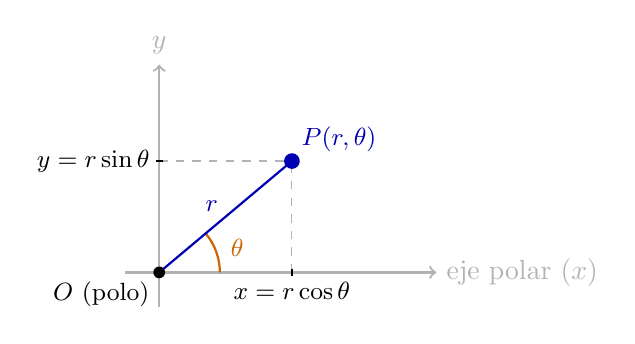
\begin{tikzpicture}[scale=2.2]
  % Ejes cartesianos
  \draw[->, thick, gray!60] (-0.2,0) -- (1.6,0) node[right] {eje polar ($x$)};
  \draw[->, thick, gray!60] (0,-0.2) -- (0,1.2) node[above] {$y$};
  % Arco del ángulo theta
  \draw[->,-,thick, orange!80!black]
    (0.35,0) arc[start angle=0, end angle=40, radius=0.35];
  \node[orange!80!black, font=\small] at (0.45, 0.14) {$\theta$};
  % Rayo OP
  \draw[thick, blue!70!black, -]
    (0,0) -- ({cos(40)},{sin(40)});
  % Proyecciones punteadas
  \draw[dashed, gray!60]
    ({cos(40)},0) node[below, black, font=\small] {$x = r\cos\theta$}
    -- ({cos(40)},{sin(40)});
  \draw[dashed, gray!60]
    (0,{sin(40)}) node[left, black, font=\small] {$y=r\sin\theta$}
    -- ({cos(40)},{sin(40)});
  % Etiqueta r sobre el rayo
  \node[blue!70!black, font=\small] at ({cos(40)/2 - 0.08},{sin(40)/2 + 0.06})
    {$r$};
  % Punto P
  \node[circle, fill=blue!70!black, inner sep=2pt]
    at ({cos(40)},{sin(40)}) {};
  \node[above right, font=\small, blue!70!black]
    at ({cos(40)},{sin(40)}) {$P(r,\theta)$};
  % Polo O
  \node[circle, fill=black, inner sep=1.5pt] at (0,0) {};
  \node[below left, font=\small] at (0,0) {$O$ (polo)};
  % Marca en el eje x
  \draw[thick] ({cos(40)}, 0.02) -- ({cos(40)}, -0.02);
  \draw[thick] (0.02, {sin(40)}) -- (-0.02, {sin(40)});
\end{tikzpicture}
\end{center}
\end{definition}

\begin{rem} Es importante tener en cuenta las siguientes observaciones:
\begin{enumerate} 
  \item No existe unicidad en los puntos de la curva, pues $(r,\theta)$, $(r,\theta + 2k\pi)$ y
    $(-r,\theta + (2k+1)\pi)$ representan el mismo punto físico.
    Esto es crucial al hallar intersecciones de curvas polares.
  \item El polo de la curva $(0,\theta)$ para cualquier $\theta$. Suele ser una
    intersección ``oculta'' que el álgebra directa no revela; verifíquelo
    siempre de forma separada.
  \item Para realizar una conversión rápida de una curva $r = f(\theta)$ a cartesiano,
    multiplique por $r$: por ejemplo, $r = 2\cos\theta \Rightarrow
    r^2 = 2r\cos\theta \Rightarrow x^2+y^2 = 2x$.
\end{enumerate}
\end{rem}

Las curvas polares tienen las siguientes propiedades:
\begin{rem} Los criterios de simetría se pueden resumir como:

\begin{enumerate} 
  \item Las curvas son simétricas respecto al \textbf{Eje polar ($\theta = 0$):} reemplazar $\theta$ por $-\theta$
        mantiene la ecuación.
  \item Las curvas son simétricas respecto al \textbf{Eje $\theta = \pi/2$:} reemplazar $\theta$ por $\pi - \theta$
        mantiene la ecuación.
  \item La curva son simétrica respecto al \textbf{polo:} reemplazar $r$ por $-r$ (o $\theta$ por $\pi + \theta$)
        mantiene la ecuación.
\end{enumerate}
\end{rem}

\begin{rem} Algunas familias notables de curvas polares se resumen como:
\begin{enumerate} 
  \item Las \textbf{Cardioides:} $r = a \pm b\cos\theta$ con $a = b$
        (forma de corazón).
  \item La \textbf{Rosa de $n$ pétalos:} $r = a\cos n\theta$;
        $n$ impar $\Rightarrow n$ pétalos, $n$ par $\Rightarrow 2n$ pétalos.
  \item La \textbf{Lemniscatas:} $r^2 = a^2\cos 2\theta$ (figura $\infty$).
  \item La \textbf{Espiral de Arquímedes:} $r = a\theta$ ($a > 0$).
\end{enumerate}
\end{rem}

% ---------------------------------------------------------------
% EJEMPLO: GALERÍA DE CURVAS POLARES NOTABLES
% ---------------------------------------------------------------
\begin{example}[Galería de curvas polares notables]
Trace e identifique las características principales de las siguientes
familias de curvas en coordenadas polares: cardioides, rosas de $n$ pétalos,
lemniscatas y la espiral de Arquímedes.

\begin{myproof}

% --- 1. CARDIOIDE ---
\textbf{Paso 1: Análisis gráfico y región — Cardioide $r = a(1+\cos\theta)$.}

Una \textbf{cardioide} ($a = b$ en $r = a + b\cos\theta$) es una curva
cerrada con un punto cúspide en el polo. Para $a = 1$: el radio máximo
$r = 2$ se alcanza en $\theta = 0$, el mínimo $r = 0$ (cúspide) en
$\theta = \pi$. Es simétrica respecto al eje polar.

\begin{center}
\begin{tikzpicture}
\begin{axis}[
  width=0.52\textwidth, height=0.52\textwidth,
  axis lines=middle, xlabel={$x$}, ylabel={$y$},
  xmin=-0.5, xmax=2.5, ymin=-1.6, ymax=1.6,
  domain=0:360, samples=300, trig format plots=deg,
  tick style={color=black}, grid=both, grid style={gray!20},
  axis equal image,
  title={Cardioide $r = 1+\cos\theta$}
]
% CORRECCIÓN: fill directo sobre el \addplot; la curva paramétrica cerrada
% se rellena automáticamente — se elimina el \path degenerado y fill between.
\addplot[thick, blue, fill=blue!20, fill opacity=0.6]
  ({(1+cos(\x))*cos(\x)}, {(1+cos(\x))*sin(\x)});
% Etiquetas notables
\node[circle, fill=red, inner sep=2pt] at (axis cs:2,0) {};
\node[above right, font=\small] at (axis cs:2,0) {$r_{\max}=2a$};
\node[circle, fill=red, inner sep=2pt] at (axis cs:0,0) {};
\node[below left, font=\small] at (axis cs:0,0) {cúspide};
\node[circle, fill=orange, inner sep=2pt] at (axis cs:0.5,0.866) {};
\node[above, font=\small] at (axis cs:0.5,0.866) {$r=1,\;\theta=\tfrac{\pi}{2}$};
\end{axis}
\end{tikzpicture}
\end{center}

\textbf{Paso 2: Elemento diferencial.}
El área encerrada usa $dA = \tfrac{1}{2}r^2\,d\theta =
\tfrac{1}{2}(1+\cos\theta)^2\,d\theta$.

\textbf{Paso 3: Límites de integración.}
Un recorrido completo: $\theta \in [0, 2\pi]$.

\textbf{Paso 4: Área total de la cardioide (con $a=1$).}
\begin{align*}
A &= \frac{1}{2}\int_0^{2\pi}(1+\cos\theta)^2\,d\theta
   = \frac{1}{2}\int_0^{2\pi}(1 + 2\cos\theta + \cos^2\theta)\,d\theta\\
  &= \frac{1}{2}\left[2\pi + 0 + \pi\right] = \frac{3\pi}{2}.
\end{align*}
Para radio genérico $a$: \;\;$\boxed{A_{\text{cardioide}} = \dfrac{3\pi a^2}{2}}$

\bigskip
% --- 2. ROSA DE n PÉTALOS ---
\textbf{Paso 1: Análisis gráfico y región — Rosa de $n$ pétalos
$r = a\cos(n\theta)$.}

Cada pétalo corresponde a un intervalo donde $r \geq 0$; su longitud
máxima es $|a|$. La regla de paridad determina el número de pétalos.
Ilustramos $r = \cos(3\theta)$ (3 pétalos, $n$ impar) y
$r = \cos(2\theta)$ (4 pétalos, $n$ par).

\begin{center}
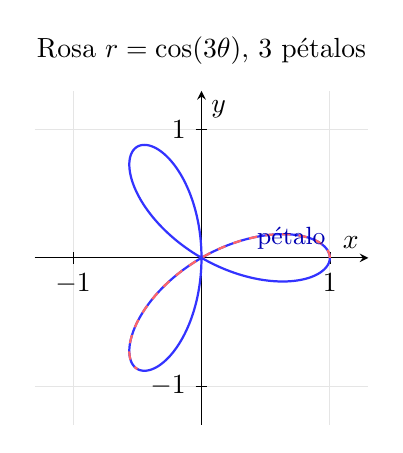
\begin{tikzpicture}
\begin{axis}[
  width=0.48\textwidth, height=0.48\textwidth,
  axis lines=middle, xlabel={$x$}, ylabel={$y$},
  xmin=-1.3, xmax=1.3, ymin=-1.3, ymax=1.3,
  domain=0:360, samples=400, trig format plots=deg,
  tick style={color=black}, grid=both, grid style={gray!20},
  axis equal image,
  title={Rosa $r=\cos(3\theta)$, 3 pétalos}
]
\addplot[thick, blue!80]
  ({cos(3*\x)*cos(\x)}, {cos(3*\x)*sin(\x)});
\addplot[thick, red!60, dashed, domain=0:60, samples=100]
  ({cos(3*\x)*cos(\x)}, {cos(3*\x)*sin(\x)});
\node[font=\small, blue!70!black] at (axis cs:0.7,0.15) {pétalo};
\end{axis}
\end{tikzpicture}
\hspace{0.5cm}
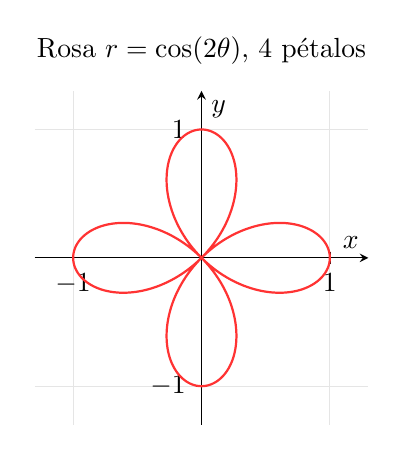
\begin{tikzpicture}
\begin{axis}[
  width=0.48\textwidth, height=0.48\textwidth,
  axis lines=middle, xlabel={$x$}, ylabel={$y$},
  xmin=-1.3, xmax=1.3, ymin=-1.3, ymax=1.3,
  domain=0:360, samples=400, trig format plots=deg,
  tick style={color=black}, grid=both, grid style={gray!20},
  axis equal image,
  title={Rosa $r=\cos(2\theta)$, 4 pétalos}
]
\addplot[thick, red!80]
  ({cos(2*\x)*cos(\x)}, {cos(2*\x)*sin(\x)});
\end{axis}
\end{tikzpicture}
\end{center}

\textbf{Paso 2: Elemento diferencial.}
$dA = \tfrac{1}{2}a^2\cos^2(n\theta)\,d\theta$.

\textbf{Paso 3 y 4: Área de un pétalo de $r = a\cos(n\theta)$.}
El pétalo principal existe para $\theta \in [-\pi/(2n),\, \pi/(2n)]$:
\begin{align*}
  A_{\text{pétalo}}
  &= \frac{a^2}{2}\int_{-\pi/(2n)}^{\pi/(2n)}\cos^2(n\theta)\,d\theta
   = \frac{a^2}{4}\int_{-\pi/(2n)}^{\pi/(2n)}(1+\cos 2n\theta)\,d\theta
   = \frac{\pi a^2}{4n}.
\end{align*}
\[
  \boxed{A_{\text{pétalo}} = \frac{\pi a^2}{4n}}
  \qquad
  \boxed{A_{\text{total}} =
    \begin{cases} n \cdot \dfrac{\pi a^2}{4n} = \dfrac{\pi a^2}{4} & n \text{ impar}\\[6pt]
                  2n \cdot \dfrac{\pi a^2}{4n} = \dfrac{\pi a^2}{2} & n \text{ par}
    \end{cases}}
\]

\bigskip
% --- 3. LEMNISCATA ---
\textbf{Paso 1: Análisis gráfico y región — Lemniscata $r^2 = a^2\cos(2\theta)$.}

La \textbf{lemniscata} tiene la forma del símbolo $\infty$. Existe solo
donde $\cos(2\theta) \geq 0$, es decir, $\theta \in [-\pi/4,\,\pi/4]$
(bucle derecho) y $\theta \in [3\pi/4,\,5\pi/4]$ (bucle izquierdo).
Su ancho máximo es $r = a$ en $\theta = 0$.

\begin{center}
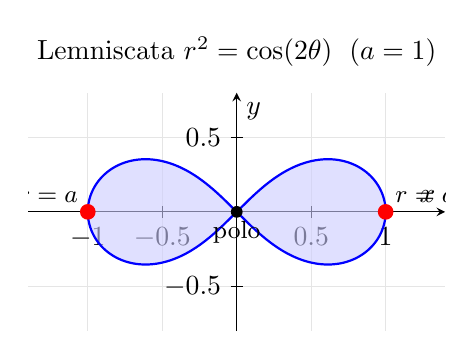
\begin{tikzpicture}
\begin{axis}[
  width=0.60\textwidth, height=0.38\textwidth,
  axis lines=middle, xlabel={$x$}, ylabel={$y$},
  xmin=-1.4, xmax=1.4, ymin=-0.8, ymax=0.8,
  tick style={color=black}, grid=both, grid style={gray!20},
  trig format plots=deg,
  axis equal image,
  title={Lemniscata $r^2 = \cos(2\theta)$\; ($a=1$)}
]
% CORRECCIÓN: cada bucle se traza como curva paramétrica cerrada con
% fill directo. En su dominio, cos(2θ)≥0, así que sqrt es segura.
% Bucle derecho: θ ∈ [-45°, 45°]; la curva sale y regresa al origen.
\addplot[thick, blue, fill=blue!20, fill opacity=0.6,
         domain=-45:45, samples=200, trig format plots=deg]
  ({sqrt(cos(2*\x))*cos(\x)}, {sqrt(cos(2*\x))*sin(\x)});
% Bucle izquierdo: θ ∈ [135°, 225°]; en ese intervalo 2θ ∈ [270°,450°],
% luego cos(2θ) ∈ [0,1] ≥ 0.
\addplot[thick, blue, fill=blue!20, fill opacity=0.6,
         domain=135:225, samples=200, trig format plots=deg]
  ({sqrt(cos(2*\x))*cos(\x)}, {sqrt(cos(2*\x))*sin(\x)});
% Puntos notables
\node[circle, fill=red, inner sep=2pt] at (axis cs:1,0) {};
\node[above right, font=\small] at (axis cs:1,0) {$r=a$};
\node[circle, fill=red, inner sep=2pt] at (axis cs:-1,0) {};
\node[above left, font=\small] at (axis cs:-1,0) {$r=a$};
\node[circle, fill=black, inner sep=1.5pt] at (axis cs:0,0) {};
\node[below, font=\small] at (axis cs:0,0) {polo};
\end{axis}
\end{tikzpicture}
\end{center}

\textbf{Paso 2: Elemento diferencial.}
$dA = \tfrac{1}{2}r^2\,d\theta = \tfrac{a^2}{2}\cos(2\theta)\,d\theta$.

\textbf{Paso 3: Límites de integración.}
Bucle derecho: $\theta \in [-\pi/4,\,\pi/4]$.

\textbf{Paso 4: Área de un bucle.}
\begin{align*}
  A_{\text{bucle}}
  &= \frac{a^2}{2}\int_{-\pi/4}^{\pi/4}\cos(2\theta)\,d\theta
   = \frac{a^2}{2}\left[\frac{\sin 2\theta}{2}\right]_{-\pi/4}^{\pi/4}
   = \frac{a^2}{2}\cdot 1.
\end{align*}
\[
  \boxed{A_{\text{bucle}} = \frac{a^2}{2}, \qquad A_{\text{total}} = a^2}
\]

\bigskip
% --- 4. ESPIRAL DE ARQUÍMEDES ---
\textbf{Paso 1: Análisis gráfico y región — Espiral de Arquímedes
$r = a\theta$ ($a>0$).}

A diferencia de las curvas cerradas anteriores, la espiral se aleja
indefinidamente del polo al crecer $\theta$. Para $a = 1/(2\pi)$, cada
vuelta completa aumenta $r$ en exactamente $1$ unidad.

\begin{center}
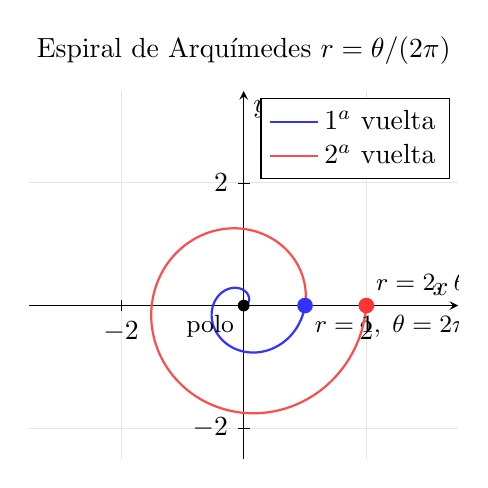
\begin{tikzpicture}
\begin{axis}[
  width=0.58\textwidth, height=0.58\textwidth,
  axis lines=middle, xlabel={$x$}, ylabel={$y$},
  xmin=-3.5, xmax=3.5, ymin=-2.5, ymax=3.5,
  domain=0:720, samples=600, trig format plots=deg,
  tick style={color=black}, grid=both, grid style={gray!20},
  axis equal image,
  title={Espiral de Arquímedes $r = \theta/(2\pi)$}
]
% Primera vuelta (0 a 360°): azul
\addplot[thick, blue!80, domain=0:360, samples=400]
  ({(x/360)*cos(x)}, {(x/360)*sin(x)});
\addlegendentry{$1^{\text{a}}$ vuelta}
% Segunda vuelta (360° a 720°): rojo
\addplot[thick, red!70, domain=360:720, samples=400]
  ({(x/360)*cos(x)}, {(x/360)*sin(x)});
\addlegendentry{$2^{\text{a}}$ vuelta}
% Puntos notables
\node[circle, fill=blue!80, inner sep=2pt] at (axis cs:1,0) {};
\node[below right, font=\small] at (axis cs:1,0)
  {$r=1,\;\theta=2\pi$};
\node[circle, fill=red!80, inner sep=2pt] at (axis cs:2,0) {};
\node[above right, font=\small] at (axis cs:2,0)
  {$r=2,\;\theta=4\pi$};
\node[circle, fill=black, inner sep=1.5pt] at (axis cs:0,0) {};
\node[below left, font=\small] at (axis cs:0,0) {polo};
\end{axis}
\end{tikzpicture}
\end{center}

\textbf{Paso 2: Elemento diferencial.}
$dA = \tfrac{1}{2}r^2\,d\theta = \tfrac{1}{2}a^2\theta^2\,d\theta$.

\textbf{Paso 3: Límites de integración.}
El área barrida en la primera vuelta completa: $\theta \in [0, 2\pi]$.

\textbf{Paso 4: Área barrida en la primera vuelta.}
\begin{align*}
  A &= \frac{a^2}{2}\int_0^{2\pi}\theta^2\,d\theta
     = \frac{a^2}{2}\left[\frac{\theta^3}{3}\right]_0^{2\pi}
     = \frac{a^2}{2}\cdot\frac{8\pi^3}{3}.
\end{align*}
\[
  \boxed{A_{\text{primera vuelta}} = \frac{4\pi^3 a^2}{3}}
\]
\end{myproof}
\end{example}

% ------------------------------------------------------------
\subsection{Área en coordenadas polares}
% ------------------------------------------------------------

Según lo que hemos estudiado, en cartesianas, $dA = y\,dx$ es el área de un
rectángulo infinitesimal. En polares, el elemento de área es un
\emph{sector circular} de ángulo $d\theta$ y radio $r$:
$dA = \frac{1}{2}r^2\,d\theta$.

\begin{theorem}[Área de una región polar]
El área de la región delimitada por la curva $r = r(\theta)$ y los rayos
$\theta = \alpha$, $\theta = \beta$ es:
\[
  A = \int_{\alpha}^{\beta} \frac{1}{2}[r(\theta)]^2\,d\theta.
\]
\end{theorem}

% --- Ejemplo: área de un pétalo de rosa ---
\begin{example}[Área de un pétalo de la rosa $r = 3\sin(3\theta)$]
Analice la curva polar $r = 3\sin(3\theta)$ y calcule el área de un solo
pétalo.

\begin{myproof}

\textbf{Paso 1: Análisis gráfico, simetría y región.}

\emph{Número de pétalos:} $n = 3$ (impar) $\Rightarrow$ \textbf{3 pétalos}
de longitud $|r|_{\max} = 3$.

\emph{Simetría:} reemplazando $\theta$ por $\pi - \theta$:
$\sin(3(\pi-\theta)) = \sin(3\pi - 3\theta) = -\sin(3\theta - 3\pi) = \sin(3\theta)$
(usando periodicidad). La curva es simétrica respecto al eje $\theta = \pi/2$.

Un pétalo se genera al variar $\theta$ en un intervalo donde $r \geq 0$.
El pétalo principal: $r = 0$ cuando $\sin(3\theta) = 0$, es decir,
$3\theta = 0$ y $3\theta = \pi$, luego $\theta \in [0, \pi/3]$.

\begin{center}
\begin{tikzpicture}
\begin{axis}[
  width=0.6\textwidth, height=0.6\textwidth,
  axis lines=middle, xlabel={$x$}, ylabel={$y$},
  xmin=-3.5, xmax=3.5, ymin=-3.5, ymax=3.5,
  domain=0:360, samples=400,
  trig format plots=deg,
  tick style={color=black}, grid=both, grid style={gray!20}
]
\addplot[thick, blue] ({3*sin(3*x)*cos(x)}, {3*sin(3*x)*sin(x)});
\addlegendentry{$r = 3\sin(3\theta)$}
% Sombreado del pétalo principal (0 a 60 grados)
\addplot[name path=petalo, orange!60, domain=0:60, samples=80]
  ({3*sin(3*x)*cos(x)}, {3*sin(3*x)*sin(x)});
\path[name path=origin] (axis cs:0,0);
\addplot[orange!30, opacity=0.6]
  fill between[of=petalo and origin, soft clip={domain=0:60}];
\node at (axis cs:1.5,1.5) {\small Pétalo};
\node at (axis cs:-1.8,2.0) {\small Pétalo};
\node at (axis cs:-1.8,-2.0) {\small Pétalo};
\end{axis}
\end{tikzpicture}
\end{center}

\textbf{Paso 2: Elemento diferencial.}
\[
  dA = \frac{1}{2}r^2\,d\theta = \frac{1}{2}[3\sin(3\theta)]^2\,d\theta
     = \frac{9}{2}\sin^2(3\theta)\,d\theta.
\]

\textbf{Paso 3: Límites de integración.}
El pétalo principal corresponde a $\theta \in [0, \pi/3]$, intervalo donde
$r = 3\sin(3\theta) \geq 0$.

\textbf{Paso 4: Evaluación.}
Utilizamos la identidad $\sin^2 u = \frac{1-\cos 2u}{2}$ con $u = 3\theta$:
\begin{align*}
  A &= \int_{0}^{\pi/3} \frac{9}{2}\sin^2(3\theta)\,d\theta
     = \frac{9}{2}\int_{0}^{\pi/3} \frac{1 - \cos 6\theta}{2}\,d\theta \\[4pt]
    &= \frac{9}{4}\left[\theta - \frac{\sin 6\theta}{6}\right]_{0}^{\pi/3}\\[4pt]
    &= \frac{9}{4}\left[\left(\frac{\pi}{3} - \frac{\sin 2\pi}{6}\right)
       - \left(0 - 0\right)\right]
     = \frac{9}{4}\cdot\frac{\pi}{3}.
\end{align*}
\[
  \boxed{A_{\text{pétalo}} = \frac{3\pi}{4}\;\text{u}^2}
\]
\end{myproof}
\end{example}

% --- Ejemplo: intersección de curvas polares ---
\begin{example}[Intersección de dos cardioides y área de la región común]
Encuentre los puntos de intersección entre las cardioides
$r = 1 + \cos\theta$ y $r = 1 - \sin\theta$, y plantee la integral para el
área de la región delimitada por $r = 1 + \cos\theta$ entre los ángulos de
cruce.

\begin{myproof}

\textbf{Paso 1: Análisis gráfico y región.}
La cardioide $r = 1 + \cos\theta$ apunta hacia la derecha; la cardioide
$r = 1 - \sin\theta$ apunta hacia abajo. Se cruzan en dos puntos visibles
y comparten el polo.

\begin{center}
\begin{tikzpicture}
\begin{axis}[
  width=0.65\textwidth, height=0.55\textwidth,
  axis lines=middle, xlabel={$x$}, ylabel={$y$},
  xmin=-2.5, xmax=2.5, ymin=-2.5, ymax=2.5,
  domain=0:360, samples=400,
  trig format plots=deg,
  tick style={color=black}, grid=both, grid style={gray!20}
]
\addplot[name path=c1, thick, blue]
  ({(1+cos(\x))*cos(\x)}, {(1+cos(\x))*sin(\x)});
\addlegendentry{$r = 1+\cos\theta$}
\addplot[name path=c2, thick, red]
  ({(1-sin(\x))*cos(\x)}, {(1-sin(\x))*sin(\x)});
\addlegendentry{$r = 1-\sin\theta$}
% Puntos de intersección
\node[circle,fill=black,inner sep=2.5pt]
  at (axis cs:{(1-0.7071)*cos(135)},{(1-0.7071)*sin(135)}) {};
\node[above left, font=\small]
  at (axis cs:{(1-0.7071)*cos(135)},{(1-0.7071)*sin(135)})
  {$P_1$};
\node[circle,fill=black,inner sep=2.5pt]
  at (axis cs:{(1+0.7071)*cos(315)},{(1+0.7071)*sin(315)}) {};
\node[below right, font=\small]
  at (axis cs:{(1+0.7071)*cos(315)},{(1+0.7071)*sin(315)})
  {$P_2$};
\end{axis}
\end{tikzpicture}
\end{center}

\textbf{Paso 2: Elemento diferencial.}
El diferencial de área en polares es un sector circular:
$dA = \tfrac{1}{2}r^2(\theta)\,d\theta$.

\textbf{Paso 3: Límites de integración.}
Igualamos:
\[
  1 + \cos\theta = 1 - \sin\theta
  \implies \cos\theta + \sin\theta = 0
  \implies \tan\theta = -1.
\]
En $[0, 2\pi)$: $\theta = \dfrac{3\pi}{4}$ y $\theta = \dfrac{7\pi}{4}$.

Además, el \textbf{polo} es intersección adicional: $r = 0$ en
$\theta = \pi$ para la primera cardioide y en $\theta = \pi/2$ para la
segunda.

\textbf{Paso 4: Evaluación del área parcial.}

Para el área barrida por la cardioide $r = 1 + \cos\theta$ entre los
ángulos de cruce:
\begin{align*}
  A_{\text{parcial}}
  &= \int_{3\pi/4}^{7\pi/4}
     \frac{1}{2}(1 + \cos\theta)^2\,d\theta \\[4pt]
  &= \frac{1}{2}\int_{3\pi/4}^{7\pi/4}
     \!\bigl(1 + 2\cos\theta + \cos^2\!\theta\bigr)\,d\theta \\[4pt]
  &= \frac{1}{2}
     \left[\theta + 2\sin\theta
           + \frac{\theta}{2} + \frac{\sin 2\theta}{4}
     \right]_{3\pi/4}^{7\pi/4} \\[4pt]
  &= \frac{9\pi}{8} - \sqrt{2}.
\end{align*}
Los puntos de intersección y el área parcial quedan determinados:
\[
  \boxed{P_1 = \!\left(1-\tfrac{\sqrt{2}}{2},\,\tfrac{3\pi}{4}\right),
  \quad
  P_2 = \!\left(1+\tfrac{\sqrt{2}}{2},\,\tfrac{7\pi}{4}\right),
  \quad \text{Polo } (0,\theta),
  \quad A_{\text{parcial}} = \tfrac{9\pi}{8} - \sqrt{2}}
\]
\end{myproof}
\end{example}

% ------------------------------------------------------------
\subsection{Longitud de arco en coordenadas polares}
% ------------------------------------------------------------

\begin{theorem}[Longitud de arco en coordenadas polares]
Si la curva está dada por $r = r(\theta)$ con $r'$ continua en
$[\alpha, \beta]$, entonces su longitud es:
\[
  s = \int_{\alpha}^{\beta}
      \sqrt{r(\theta)^2 + [r'(\theta)]^2}\;d\theta.
\]
\begin{proof}
Usando las relaciones $x = r\cos\theta$, $y = r\sin\theta$ y diferenciando:
$x' = r'\cos\theta - r\sin\theta$, $y' = r'\sin\theta + r\cos\theta$.
Entonces
$(x')^2 + (y')^2 = (r')^2(\cos^2\theta + \sin^2\theta)
 + r^2(\sin^2\theta + \cos^2\theta) = (r')^2 + r^2$.
Sustituyendo en la fórmula paramétrica se obtiene el resultado.
\end{proof}
\end{theorem}

\begin{example}[Longitud de la espiral de Arquímedes]
Calcule la longitud de la espiral de Arquímedes $r = \theta$ para
$\theta \in [0, 2\pi]$.

\begin{myproof}

\textbf{Paso 1: Análisis gráfico y región.}
La espiral parte del polo ($r=0$ cuando $\theta=0$) y se aleja de forma
lineal: a mayor ángulo, mayor radio. El arco cuya longitud calcularemos
va desde el polo hasta el punto $(2\pi, 0)$ en cartesianas, después de
una vuelta completa.

\begin{center}
\begin{tikzpicture}
\begin{axis}[
  width=0.60\textwidth, height=0.60\textwidth,
  axis lines=middle, xlabel={$x$}, ylabel={$y$},
  xmin=-7, xmax=7, ymin=-7, ymax=7,
  domain=0:720, samples=600,
  trig format plots=deg,
  tick style={color=black},
  grid=both, grid style={gray!20},
  axis equal image,
  title={Espiral de Arquímedes $r = \theta$\quad($\theta$ en rad)}
]
\addplot[thick, blue!80, domain=0:360, samples=500]
  ({(x*pi/180)*cos(x)}, {(x*pi/180)*sin(x)});
\addlegendentry{$r=\theta,\;\theta\in[0,2\pi]$}
\node[circle, fill=black, inner sep=2pt] at (axis cs:0,0) {};
\node[below left, font=\small] at (axis cs:0,0) {polo $\theta=0$};
\node[circle, fill=red, inner sep=2.5pt]
  at (axis cs:{2*pi}, 0) {};
\node[above right, font=\small]
  at (axis cs:{2*pi}, 0) {$\theta=2\pi,\;r=2\pi$};
\node[circle, fill=orange, inner sep=2pt]
  at (axis cs:0, {pi/2}) {};
\node[right, font=\small]
  at (axis cs:0, {pi/2}) {$\theta=\tfrac{\pi}{2}$};
\node[circle, fill=orange, inner sep=2pt]
  at (axis cs:{-pi}, 0) {};
\node[above, font=\small]
  at (axis cs:{-pi}, 0) {$\theta=\pi$};
\draw[dashed, gray!70]
  (axis cs:0,0) -- (axis cs:{(pi/4)*cos(45)},{(pi/4)*sin(45)});
\node[font=\small, gray!60!black]
  at (axis cs:0.6, 0.85) {$r=\theta$};
\end{axis}
\end{tikzpicture}
\end{center}

\textbf{Paso 2: Elemento diferencial de arco.}
Para $r(\theta) = \theta$ se tiene $r'(\theta) = 1$, luego:
\[
  ds = \sqrt{r^2 + (r')^2}\,d\theta = \sqrt{\theta^2 + 1}\,d\theta.
\]

\textbf{Paso 3: Límites de integración.}
Una vuelta completa corresponde a $\theta \in [0,\,2\pi]$, por lo que:
\[
  s = \int_{0}^{2\pi}\sqrt{\theta^2 + 1}\;d\theta.
\]

\textbf{Paso 4: Antiderivada mediante sustitución trigonométrica.}

Calculamos primero la antiderivada indefinida. Sea $\theta = \tan u$,
de modo que $d\theta = \sec^2 u\,du$ y
$\sqrt{\theta^2 + 1} = \sqrt{\tan^2 u + 1} = \sec u$ (con $\sec u > 0$):
\[
  \int\sqrt{\theta^2+1}\,d\theta
  = \int \sec u \cdot \sec^2 u\,du
  = \int \sec^3 u\,du.
\]

\textbf{Paso 4a: Integral de $\sec^3 u$ por partes.}
Tomamos $p = \sec u$ y $dq = \sec^2 u\,du$, de donde
$dp = \sec u\tan u\,du$ y $q = \tan u$:
\begin{align*}
  \int \sec^3 u\,du
  &= \sec u\tan u - \int \sec u\tan^2 u\,du \\
  &= \sec u\tan u - \int \sec u\,(\sec^2 u - 1)\,du \\
  &= \sec u\tan u - \int \sec^3 u\,du + \int \sec u\,du.
\end{align*}
Despejando $\int \sec^3 u\,du$:
\begin{align*}
  2\int \sec^3 u\,du
  &= \sec u\tan u + \int \sec u\,du
   = \sec u\tan u + \ln|\sec u + \tan u| + C,\\[4pt]
  \int \sec^3 u\,du
  &= \frac{\sec u\tan u + \ln|\sec u + \tan u|}{2} + C.
\end{align*}

\textbf{Paso 4b: Regreso a la variable $\theta$.}
De la sustitución $\theta = \tan u$ se tiene $\sec u = \sqrt{\theta^2+1}$
y $\tan u = \theta$, luego:
\[
  \int\sqrt{\theta^2+1}\,d\theta
  = \frac{\theta\sqrt{\theta^2+1} + \ln\!\left(\theta + \sqrt{\theta^2+1}\right)}{2}
    + C.
\]
(Nótese que $\theta + \sqrt{\theta^2+1} > 0$ para todo $\theta$, por lo
que se suprime el valor absoluto.)

\textbf{Paso 5: Evaluación en $[0,\,2\pi]$.}
\begin{align*}
  s
  &= \left[\frac{\theta\sqrt{\theta^2+1}
             + \ln\!\left(\theta + \sqrt{\theta^2+1}\right)}{2}
    \right]_{0}^{2\pi} \\[6pt]
  &= \frac{2\pi\sqrt{4\pi^2+1}
           + \ln\!\left(2\pi + \sqrt{4\pi^2+1}\right)}{2}
   - \frac{0\cdot 1 + \ln(0 + 1)}{2} \\[6pt]
  &= \pi\sqrt{4\pi^2+1}
     + \frac{\ln\!\left(2\pi + \sqrt{4\pi^2+1}\right)}{2}
     - 0.
\end{align*}
Numéricamente: $\sqrt{4\pi^2+1} \approx 6{,}361$, \;
$2\pi + 6{,}361 \approx 12{,}645$, luego
$s \approx \pi \cdot 6{,}361 + \tfrac{1}{2}\ln(12{,}645)
 \approx 19{,}98 + 1{,}27 \approx 21{,}26$ u.
\[
  \boxed{s = \pi\sqrt{4\pi^2+1}
           + \frac{1}{2}\ln\!\left(2\pi+\sqrt{4\pi^2+1}\right)
           \approx 21{,}26\;\text{u}}
\]
\end{myproof}
\end{example}


\section{Problemas propuestos}


\begin{prob}
Para cada curva dada en forma paramétrica, elimine el parámetro para obtener
la ecuación cartesiana equivalente e identifique la curva resultante. Trace un
bosquejo de la gráfica indicando con flechas la dirección de recorrido a medida
que el parámetro $t$ crece.
\begin{enumerate}
    \item $x = 6t + 2,\quad y = 2t;\quad -\infty < t < \infty$
    \item $x = 4t^2,\quad y = 4t;\quad -1 \leq t \leq 2$
    \item $x = 2\sec t,\quad y = \tan t;\quad
          -\dfrac{\pi}{2} < t < \dfrac{\pi}{2}$
    \item $x = 4\sin t - 2,\quad y = 3\cos t + 1;\quad 0 \leq t \leq 2\pi$
\end{enumerate}
\end{prob}

\begin{prob}
Para cada curva paramétrica, calcule la derivada $\dfrac{dy}{dx}$ y determine
la ecuación de la recta tangente en el punto correspondiente al valor $t = 0$
del parámetro.
\begin{enumerate}
    \item $x = 3e^{-t},\quad y = \dfrac{1}{2}e^{t}$
    \item $x = 2t^3 - 4t + 7,\quad y = t + \ln(t + 1)$
\end{enumerate}
\end{prob}

\begin{prob}
Considere la curva paramétrica definida por $x = t^2 - 4$ e $y = t^3 - 3t$.
\begin{enumerate}
    \item Determine las coordenadas cartesianas $(x, y)$ de todos los puntos
          de la curva en los que la recta tangente es horizontal.
    \item Calcule la segunda derivada $\dfrac{d^2y}{dx^2}$ y evalúela en
          $t = 2$ para determinar la concavidad de la curva en ese punto.
\end{enumerate}
\end{prob}

\begin{prob}
La cicloide está definida paramétricamente por $x = t - \sin t$ e
$y = 1 - \cos t$, para $0 \leq t \leq 2\pi$. Plantee y evalúe la integral
definida que representa el área de la región plana acotada superiormente
por un arco completo de la cicloide e inferiormente por el eje $x$.
\end{prob}

\begin{prob}
Plantee y evalúe la integral definida que representa la longitud de arco de
cada curva paramétrica en el intervalo indicado.
\begin{enumerate}
    \item $x = 1 + t^{3/2},\quad y = 2 + t^{3/2},\quad 0 \leq t \leq 9$
    \item $x = \cos t + t\sin t,\quad y = \sin t - t\cos t,\quad
          0 \leq t \leq 2\pi$
\end{enumerate}
\end{prob}

\begin{prob}
Halle el área de la superficie de revolución generada al hacer girar el arco
de la curva paramétrica $x = \cos^3 t$, $y = \sin^3 t$, con
$0 \leq t \leq \pi/2$, alrededor del eje $x$. Incluya el planteamiento
completo de la integral antes de proceder con su evaluación.
\end{prob}


\begin{prob}
Para cada ecuación polar, obtenga una ecuación cartesiana equivalente e
identifique la curva resultante (recta, circunferencia, cónica, etc.).
Incluya un bosquejo de la curva en el plano.
\begin{enumerate}
    \item $r = 6\cos\theta$
    \item $r = \dfrac{3}{\cos\theta}$
    \item $r^2\cos 2\theta = 9$
    \item $r^2 - 6r(\cos\theta + \sin\theta) + 9 = 0$
\end{enumerate}
\end{prob}

\begin{prob}
Calcule la pendiente de la recta tangente a la curva polar
$r = 3 + 3\cos\theta$ en el punto donde $\theta = \dfrac{\pi}{6}$.
\end{prob}

\begin{prob}
Dada la curva polar $r = 1 - \sin\theta$, determine las coordenadas polares
$(r,\theta)$ de todos los puntos de la curva en los que la recta tangente es
horizontal. Considere $0 \leq \theta < 2\pi$ y justifique el tratamiento
analítico de los posibles puntos en que $dy/d\theta$ y $dx/d\theta$ se
anulan simultáneamente.
\end{prob}

\begin{prob}
Determine los límites de integración adecuados y calcule el área de la región
indicada en cada caso.
\begin{enumerate}
    \item El área de uno de los bucles de la lemniscata $r^2 = 4\cos(2\theta)$.
          Establezca los ángulos exactos en los que $r = 0$ para fijar los
          límites de integración.
    \item El área encerrada por un solo pétalo de la rosa polar
          $r = 3\sin(3\theta)$. Indique el número total de pétalos y
          justifique la elección del intervalo de integración.
\end{enumerate}
\end{prob}

\begin{prob}
Utilice la integración en coordenadas polares para resolver los siguientes
problemas de áreas.
\begin{enumerate}
    \item Determine el área total de la región acotada por el cardioide
          $r = 5 - 5\cos\theta$.
    \item Encuentre los puntos de intersección de $r = 5\sin\theta$ y
          $r = 2 + \sin\theta$. Calcule el área de la región que se
          encuentra dentro del círculo $r = 5\sin\theta$ y fuera del
          caracol $r = 2 + \sin\theta$.
\end{enumerate}
\end{prob}

\begin{prob}
Plantee y evalúe la integral que representa la longitud de arco exacta de
cada curva polar en el intervalo indicado.
\begin{enumerate}
    \item La espiral logarítmica $r = e^{2\theta}$, desde $\theta = 0$
          hasta $\theta = 2\pi$.
    \item El cardioide $r = a(1 - \cos\theta)$, para $0 \leq \theta \leq 2\pi$.
          \emph{Sugerencia:} aplique la identidad de ángulo mitad
          $1 - \cos\theta = 2\sin^2(\theta/2)$ para resolver la raíz
          cuadrada del integrando.
\end{enumerate}
\end{prob}



